\documentclass{article}
\usepackage[utf8]{inputenc}
\usepackage{physics}
\usepackage{amsmath}
\usepackage{amssymb}
\usepackage{graphicx}
\usepackage{enumitem}
\usepackage{hyperref}
\hypersetup{
    colorlinks=true,    
    urlcolor=blue,
}


\title{Homework 6: Policy Gradient Reinforcement Learning}
\date{Due November 22nd, 2019 at 11:59pm}
\author{CS 1470/2470}
\begin{document}

\maketitle

\section{Conceptual Questions}
\begin{enumerate}

  \item What are some of the differences between the REINFORCE algorithm (Monte-Carlo method) and the Advantage Actor Critic? (3-5 sentences) 
  
    \textit{Hint: Remember to discuss the differences in the loss functions between the two methods} \\
    \textit{Hint: Discuss the variance differences of the gradient estimates}

    \item In reinforcement learning, we often discuss the exploration-exploitation tradeoff. We mush balance acquiring new knowledge about our environment (exploration) while simultaneously trying to maximize our return (utilizing all the knowledge we've collected thus far). How do policy gradient methods automatically perform this tradeoff? (2-4 sentences)
    
    \item What advantages do policy gradient methods have over deep $Q$ learning methods? What advantages do deep $Q$ learning methods have over policy gradient methods? (3-5 sentences)

\end{enumerate}


\section{Ethical Implications}
\begin{enumerate}
\item One of the most important and quickly-developing uses of reinforcement learning is for self-driving vehicles. These autonomous vehicles stand to revolutionize industries like ride-sharing, trucking, and package delivery, potentially automating over 4 million currently existing jobs. Check out some news reports on this issue, ranging from the \href{https://www.cnbc.com/2017/05/22/goldman-sachs-analysis-of-autonomous-vehicle-job-loss.html}{pessimistic} to the \href{https://www.wired.com/story/guide-self-driving-cars/}{neutral} to the \href{https://avworkforce.secureenergy.org/wp-content/uploads/2018/06/Americas-Workforce-and-the-Self-Driving-Future_Realizing-Productivity-Gains-and-Spurring-Economic-Growth.pdf}{optimistic} (pp. 10-12).

Do the potential economic benefits of autonomous vehicles outweigh the labor costs? Why or why not? (2-4 sentences)

\item Within the realm of speculative fiction, much has been written about the obligations of scientists to the sentient beings that they create (Mary Shelley’s \href{https://www.planetebook.com/free-ebooks/frankenstein.pdf}{\textit{Frankenstein}}, Ted Chiang’s \href{https://cpb-us-w2.wpmucdn.com/voices.uchicago.edu/dist/8/644/files/2017/08/Chiang-Lifecycle-of-Software-Objects-q3tsuw.pdf}{\textit{Lifecycle of Software Objects}}, and \textbf{many} others). Some computer scientists and philosophers have argued that with recent advances, RL algorithms represent a kind of sentience, and that humans should take the suffering of RL algorithms into account. This has even led to the creation of groups like \href{http://petrl.org/}{People for the Ethical Treatment of Reinforcement Learners}.

Do you agree or disagree with this viewpoint? Do we as humans currently have moral obligations to treat RL algorithms ethically? Why or why not? If not, what would change your mind? (3-5 sentences)
    
\end{enumerate}

\section{CS2470-only Questions}

\begin{enumerate}

    \item 
    RL agents struggle when the MDP they are trying to solve requires a long sequence of coordinated actions before any reward signal is received. This motivates the practice of “reward shaping,” or trying to design reward functions that somehow gradually reward an agent for making progress toward its ultimate goal. A classic example of this phenomenon occurs in the Atari game Montezuma’s Revenge. The included figure shows the starting screen of the first level of this game.
    
    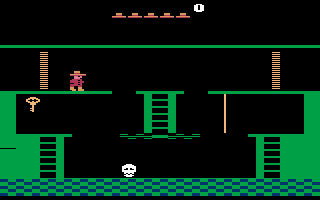
\includegraphics[]{figs/image.png}
    
    \begin{enumerate}[label=(\alph*)]
        \item Assume that the agent receives a reward of 1 (i.e. a score increment of 1) when it retrieves the key located on the left part of the screen. In order to get to this key, the agent must learn to jump across platform gaps, climb down a latter, jump onto a hanging rope, fall off the rope, avoid the moving skull enemy, and climb up the final ladder to the key. Design a reward function that will encourage the agent to get to the key as quickly as possible, while avoiding death (assume you have access to the complete state of the game).
        \item
        For an actual RL agent trying to play Montezuma’s revenge, the situation is more dire: the only input the agent can see are pixels, and obtaining the key actually does not confer any reward. Rather, reward is only obtained if the agent obtains the key, moves to a different screen to the left or right of the current screen, and uses the key to unlock something. Can you think of possible reward functions that might encourage this behavior (in this case, you only have access to the raw game pixels).
        \item
        If your strategy from part 2 was specific to Montezuma’s Revenge: now can you think of ways it might be generalized to apply to any Atari game (i.e. any MDP where the inputs are pixels, the actions are discrete controller inputs, and the reward is game score)?
    \end{enumerate}

    \item The objective function for policy gradients is defined as: 
    $$J(\theta) = \mathbb{E}[\sum_{t=0}^{T - 1} r_{t+1}]$$
    
    Derive the policy gradient i.e $\nabla_{\theta}J(\theta)$
    
    \textit{Hints:}
    \begin{enumerate}
        \item \textit{Rewrite the expectation using your policy $\pi_{\theta}$}
        \item \textit{Write out the objective with respect to an arbitrary trajectory}
        \item \textit{Recall $\frac{d}{{dx}}\log \left(f(x) \right) = \frac{f'(x)}{f(x)}$}
        
    \end{enumerate}
\end{enumerate}
\end{document}
